%!TEX root = index.tex
\chapter[Requisitos]{Requisitos}
\label{chap:requisitos}

A partir dos objetivos deste Trabalho de Conclusão de Curso, é possível extrair os requisitos funcionais do sistema de recomendação. Esses requisitos ditam principalmente sobre a escalabilidade e o desempenho das recomendações do sistema.

Como as sugestões serão calculadas com antecedência, não há necessidade para uma elevada taxa de recomendações por período de tempo (\textit{throughput}). Deseja-se contudo que o sistema possa gerar todas as recomendações para um banco de dados de cem mil clientes em uma hora, isto é, que tenha \textit{throughput} mínimo de 28 recomendação por segundo. Os sistemas de recomendação tradicionais possuem \textit{throughput} de cerca de 500 recomendações por segundo, mas operam em servidores dedicados de maior potência computacional \cite{sarwar2001item}. 

A fim de poder estabelecer uma base comparativa entre o sistema proposto \textit{UI} e os sistemas de referência \textit{FW} e \textit{UP}, serão utilizados os mesmos indicadores de desempenho dos artigos-base: precisão, abrangência e medida $F_1$ \cite{symeonidis2007feature,debnath2008feature}. Precisão é a porcentagem de casos corretamente preditos em relação ao tamanho da lista de recomendações. Abrangência é a razão entre o número de itens corretamente preditos e daqueles que foram efetivamente avaliados pelo usuário. A medida $F_1$, por sua vez, é a média harmônica entre precisão e
abrangência.

Todas essas métricas são dependentes dos diversos parâmetros do problema, como do tamanho da lista de recomendações $N$, da quantidade de vizinhos mais próximos $k$, e principalmente do banco de dados de teste. Como os artigos de referência não os disponibilizaram integralmente, serão estimados os valores de precisão, abrangência e medida $F_1$ para o banco de dados da dupla. 

Espera-se que a precisão, abrangência e consequentemente a medida $F_1$ sejam maiores que 20\%. Esses valores foram escolhidos por serem superiores aos de algoritmos puramente baseados em conteúdo ou em filtragem colaborativa \cite{symeonidis2007feature,debnath2008feature}. Na prática, o resultado mais importante é a comparação entre os três métodos para um banco de dados de referência. 

Neste trabalho o \textit{benchmarking} é feito por meio da união de dois bancos amplamente utilizados na comunidade científica de Sistemas de Recomendação. O primeiro, denominado MovieLens 100k, é composto de 100 000 avaliações (valores inteiros de 1 a 5) de 943 usuários para 1682 filmes \cite{movielensdataset}. Além disso, cada usuário (idade, sexo, profissão, logradouro) avaliou pelo menos 20 filmes (categoria, ano de publicação). O segundo banco de dados é extraído do Internet Movie Database (IMDB), e possui 28 819 filmes. Esse banco está presente na biblioteca \texttt{ggplot2} da linguagem de programação R \cite{moviesggplot2dataset}. A união desses dois bancos é denominada 100k-IMDB, e a metodologia para essa união está descrita na Seção \ref{sec:modelamento_e_simula_o}.

Os requisitos funcionais são suportados por requisitos não-funcionais, e estes são determinados pelas restrições sobre o projeto ou execução, tais como desenvolvimento e confiabilidade.

O sistema de recomendação deverá poder ser utilizado por qualquer e-commerce que disponha de um banco de dados de clientes, produtos e histórico de compras, desde que o formato de entrada, a ser especificado no Capítulo \ref{chap:resultados}, seja seguido.

Além disso o sistema deverá ser desenvolvido em tecnologias abertas (\textit{open source}) que tenham um alto número de colaboradores, como o sistema de gestão de banco de dados MySQL ou a linguagem de programação estatística R, a fim de torná-lo reutilizável por alunos ou e-commerces interessados.

Por fim, o sistema de recomendação deverá ser escalável e flexível no sentido de poder operar igualmente bem tanto em pequenas quanto em grandes bases de dados.

Apesar serem importantes parâmetros de um sistema de recomendação, a taxa de recomendações por período de tempo e a escalabilidade estão intimamente relacionados ao orçamento do projeto. Pode-se obter virtualmente qualquer \textit{throughput} desejado, contanto que haja investimento equivalente em infra-estrutura computacional. O mesmo não é válido para os parâmetros de qualidade da recomendação, que dependem tão somente dos algoritmos de sugestão. Neste trabalho, assumimos que o sistema de operará em microcomputadores pessoais, e por isso o requisito funcional \textit{throughput} se faz necessário.

Com os requisitos do sistema de recomendação definidos, devemos estruturar o seu relacionamento com o administrador do sistema. Para isto determinamos seus casos de uso, classes e atividades.

\section{Diagrama de Casos de Uso} % (fold)
\label{sec:Diagrama de Casos de Uso}

Os casos de uso se dividem em \textit{Avaliar Performance}, \textit{Configurar Banco de Dados}, \textit{Recomendar UI}, \textit{Recomendar UP}, \textit{Recomendar FW}.

O caso de Uso \textit{Avaliar Performance}, para avaliar a performance do sistema de recomendação. \textit{Avaliar Performance} se relaciona com outros 3 casos de uso. O primeiro deles, \textit{Mascarar Dados}, serve para mascarar dados de alguns usuários-teste na matriz de avaliações. Para, após, compará-los às recomendações calculadas pelo sistema. O segundo caso, \textit{Dividir Banco de Treino}, tem o objetivo de dividir o banco de dados em dois, um para o aprendizado do sistema e o segundo para testes. O terceiro caso, \textit{Devolver Indicadores}, torna os indicadores de performance acessíveis ao administrador do sistema.

O caso de uso \textit{Configurar Banco de Dados} tem a utilidade de converter o banco de dados de entrada em matrizes. O caso \textit{Ler Itens}, é o encarregado de ler o arquivo de itens fornecido pelo banco de dados, assim como \textit{Ler Usuários} e \textit{Ler Histórico} são para usuários e histórico. Os casos de uso \textit{Gerar Matriz de Atributos} e \textit{Gerar Matriz de Avaliação} constroem as matrizes de acordo com dados lidos pelos casos de uso de leitura.

Já os casos de uso \textit{Recomendar UI}, \textit{Recomendar UP} e \textit{Recomendar FW}, são os cacsos de uso em que se geram as recomendações pelos métodos baseados na correlação usuário-item, no perfil de usuários e na ponderação de atributos respectivamente. O método de recomendação baseado na ponderação de atributos necessita de outros 3 casos de uso, o \textit{Normalizar Matriz}, onde se normaliza as colunas da matriz de distância entre atributos. Esta distância entre atributos é calculada pelos dois outros casos de uso, \textit{Fazer Delta de Kronecker} e \textit{Fazer Indice Jaccard}.

 Estes casos de uso foram representados no diagrama de casos de uso (Figura \ref{fig:Diagrama de Casos de Uso}).

 \begin{figure}[htp]
    \begin{center}
    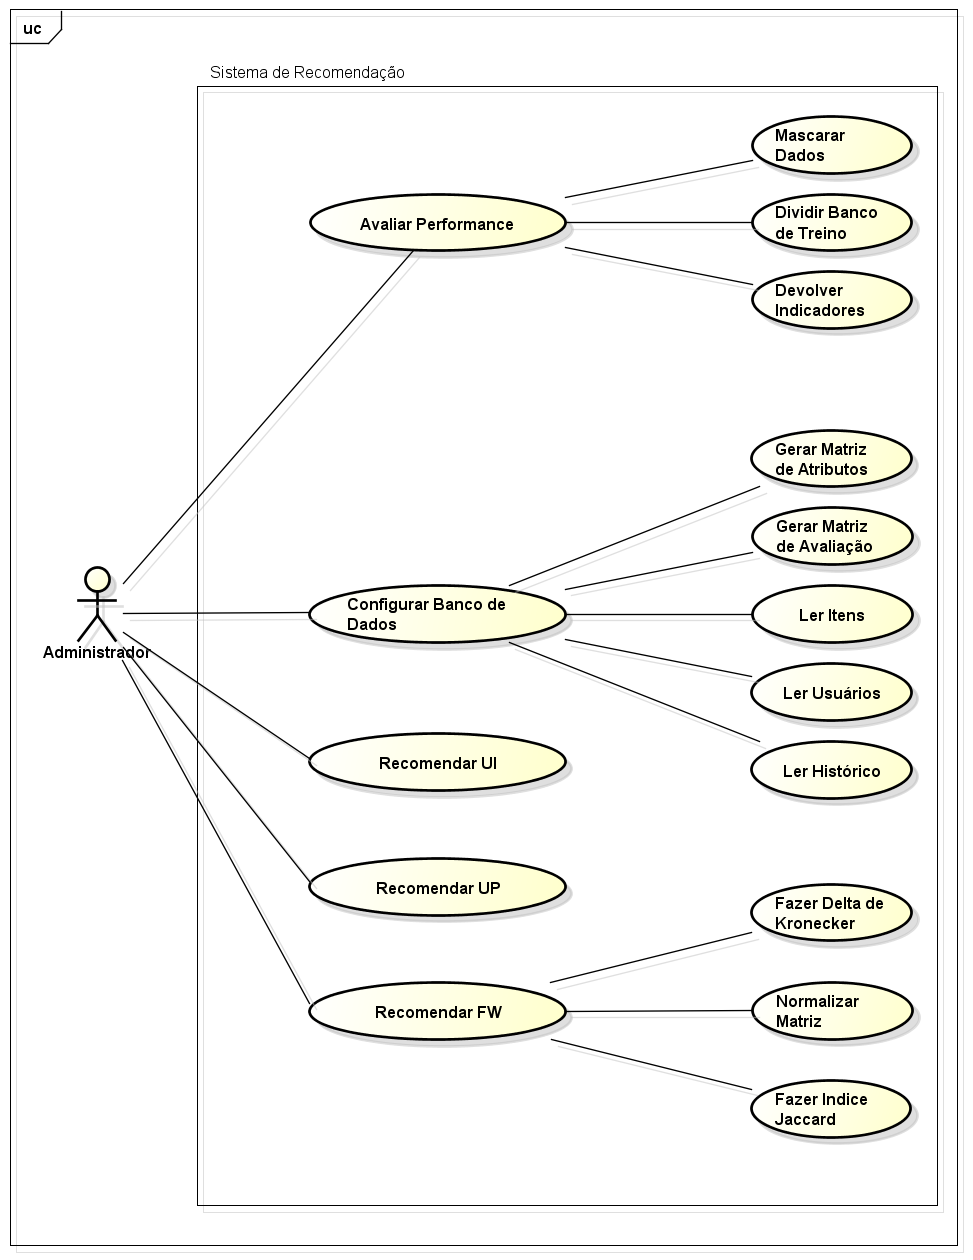
\includegraphics[width=1\textwidth]{img/CasosDeUso}
    \end{center}
    \label{fig:Diagrama de Casos de Uso}
    \caption{Diagrama de casos de uso representando os relacionamentos entre o administrador e o sistema de recomendações.}
\end{figure}

\section{Diagrama de Atividades} % (fold)
\label{sec:Diagrama de Atividades}

Para representar o fluxo de informação foi considerado o diagrama de atividades. Assim é possível visualizar os processos que vão desde a informação fornecida pelo usuário à geração de recomendações.

O primeiro diagrama de atividade (Figura \ref{fig:Diagrama de Atividades - Registro de Avaliacao}) representa o registro de uma avaliação por parte do cliente, onde o cliente solicita o item para visualizá-lo, a plataforma Web faz o pedido de informações ao banco de dados. O banco de dados devolve as informações pedidas e a plataforma o exibe no dispositivo do cliente. Após a visualização o cliente avalia o item, a plataforma web informa ao banco de dados sobre a avaliação que a registra e a plataforma Web confirma a avaliação finalizando o processo.

 \begin{figure}[htp]
    \begin{center}
    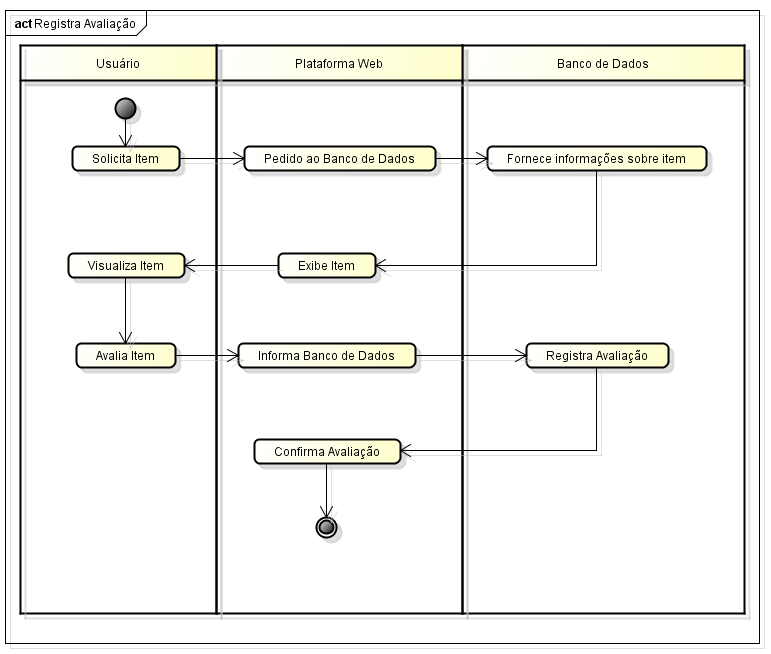
\includegraphics[width=1\textwidth]{img/Atividade_Usuario}
    \end{center}
    \label{fig:Diagrama de Atividades - Registro de Avaliacao}
    \caption{Diagrama Atividades - Registro de Avaliação}
\end{figure}

O segundo diagrama (Figura \ref{fig:Diagrama de Atividades - Recomendacao}), representa o fluxo de informação desde o pedido de uma recomendação pela plataforma web até a finalização da atividade pelo cliente. O primeiro passo é o pedido de uma recomendação, ao banco de dados, pela plataforma web. O banco de dados envia as informações necessárias para o sistema de recomendação que de acordo com as regras pré-estabelecidas as calcula e retorna para o banco de dados. O banco de dados registra estas recomendações e informa a plataforma web, que envia a recomendação ao usuário. O usuário avalia o item recomendado e finaliza o processo. 


 \begin{figure}[htp]
    \begin{center}
    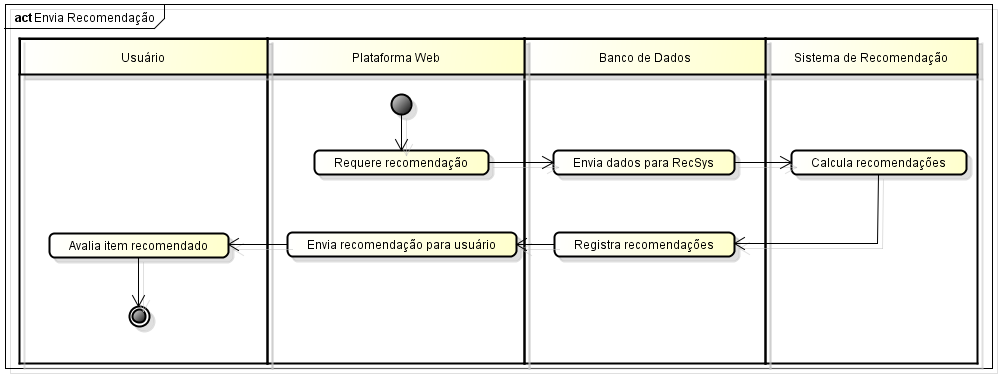
\includegraphics[width=1\textwidth]{img/Atividade_Recomendacao}
    \end{center}
    \label{fig:Diagrama de Atividades - Recomendacao}
    \caption{Diagrama Atividades - Gerar Recomendação}
\end{figure}